\documentclass[11pt]{article}

\usepackage{microtype}
\usepackage{amsmath}
\usepackage{float}
\usepackage[colorlinks, urlcolor = blue]{hyperref}

\usepackage{graphicx}
\usepackage{caption}
\usepackage{subcaption}
\usepackage{hyperref}

\title{\textbf{Motion estimation}}
\author{ Moritz Loos 112385 }
\date{ Winter term 2014/15 }

\begin{document}
	%\bibliographystyle{acm}%Association for Computiny Machinery  bibliograhpic style
	\bibliographystyle{unsrt}
	
	\maketitle

	\section{Abstract}
	The goal of the project was to estimate the motion of a UAV using a stereo camera system with help of the optical flow in the stereo images.

	\section{Introduction}
	The term optical flow describes the tracking of points from one image to another. Generally there are two possible approaches:
	At first we try to track every single pixel from frame to frame (called optical-field matching in the following). In order to reduce the number of points to track we can use an interval to determine points to track (e.g. tracking every tenth pixel within every frame). The second approach would be tracking defined features instead of every pixel in every frame(feature-based matching).
	
	\begin{figure}[H]
	        \centering
	        %LINKS
	        \begin{subfigure}[b]{0.45\textwidth}
	                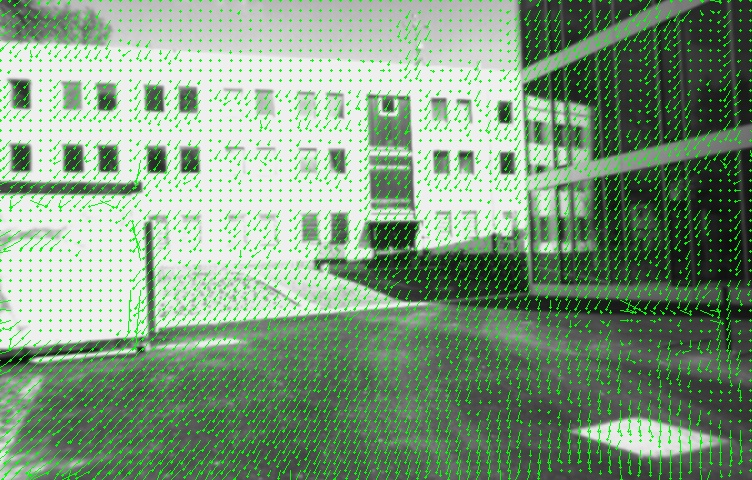
\includegraphics[width=1.0\textwidth]{images/farneback.jpg}
	                \caption{optical-field-matching}
	        \end{subfigure}\hfill 
	        %RECHTS
	        \begin{subfigure}[b]{0.45\textwidth}
	                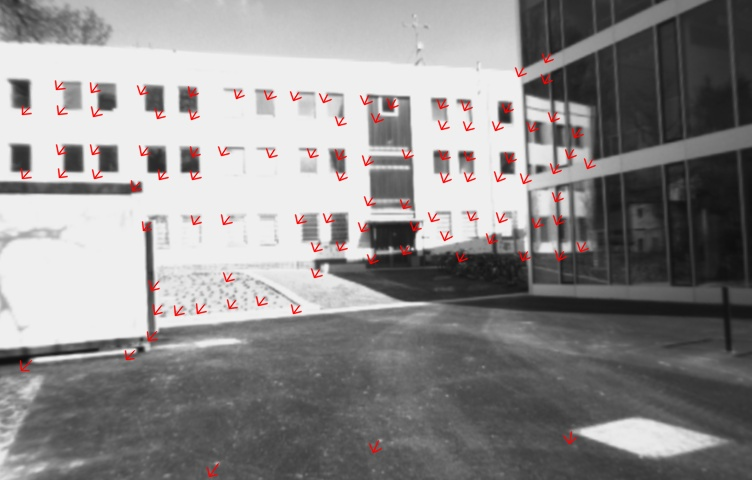
\includegraphics[width=1.0\textwidth]{images/feature-based-matching.jpg}
	                \caption{feature-based-matching}
	        \end{subfigure}
	\end{figure}
	
	Using optical-field matching the number of points is much higher than in feature-based matching. Also the distribution of points is much better. On the other side the number of outliers as well as the computational effort are growing.

	In order to make the framework portable and stable (for the future use as a method for realtime flight-path detection) the basis is a feature-based matching algorithm.

	Unfortunately a simple mapping of optical flow vectors to the motion of a camera is just possible when some special constraints are fulfilled \cite{BewegungsanalyseMuenchen}.
	
	\begin{enumerate}
	  \item The scene has to be static
	  \item The scene has to be parallel to the image plane of the camera
	  \item The scenes height has to be predefined.
	\end{enumerate}
	
	That means the camera has to look down permanently (see figure 2).

	\begin{figure}[H]
		\centering
		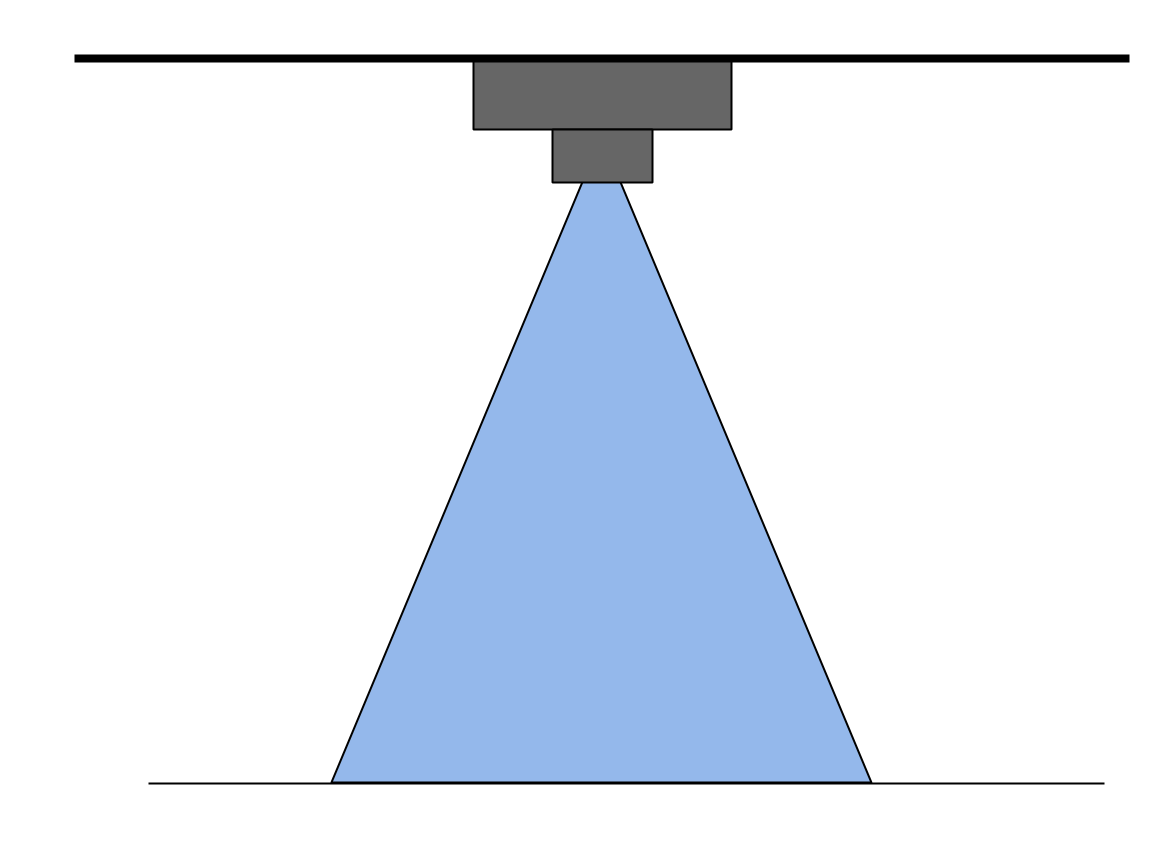
\includegraphics[width=0.5\textwidth]{images/look_down.png}
		\caption{camera constraint}
	\end{figure}

	
	If all these constraints are fulfilled it is possible to estimate the motion of the camera just using the length and the direction of the optical flow vectors.

	\begin{figure}[H]
	        \centering
	        %LINKS
	        \begin{subfigure}[b]{0.35\textwidth}
	                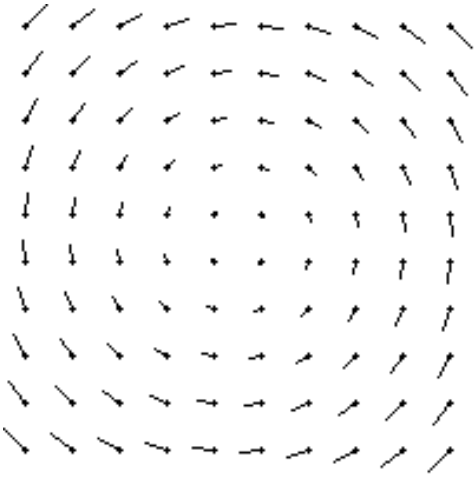
\includegraphics[width=1.0\textwidth]{images/rotation.png}
	                \caption{rotation}
	        \end{subfigure}\hfill 
	        %RECHTS
	        \begin{subfigure}[b]{0.35\textwidth}
	                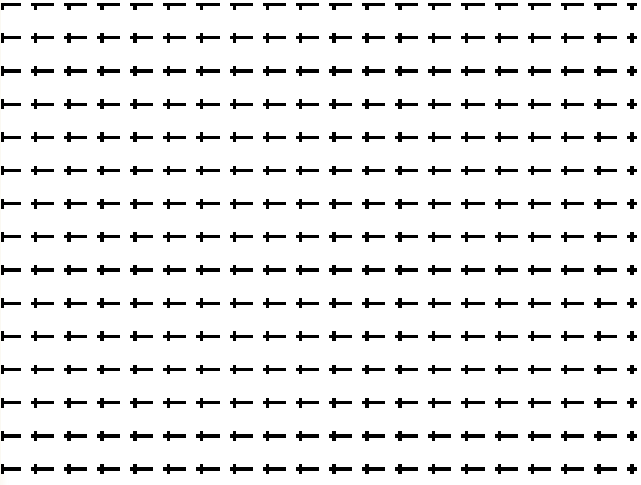
\includegraphics[width=1.0\textwidth]{images/translation.png}
	                \caption{translation}
	        \end{subfigure}
	\caption{optical flow \cite{BewegungsanalyseMuenchen}}

	\end{figure}

	As it is not possible for us to hold this constraints we had to find other approaches.

	\section{Settings}
	The system we are using is a calibrated stereo rig \cite{malik-hiller-2015} and all values are defined like described in figure 4. Where $P$ represents the projection matrix of the current camera($P_L$ is defined as the projection matrix from the left camera in previous frame i-1 to the left camera in current frame i). $C$ describes the previous respectively current camera image.
	
	\begin{figure}[H]
		\centering
		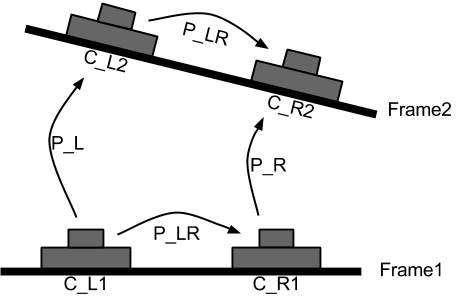
\includegraphics[width=0.7\textwidth]{images/camera_setup.png}
		\caption{camera setup}
	\end{figure}
	
	\newpage
	
	\section{Visual odometry}
	In order to estimate the motion we need to find corresponding points in all 4 images. Our approach for performing visual odometry is represented in figure 5 and is explained in the following.
	
	\begin{figure}[H]
		\centering
		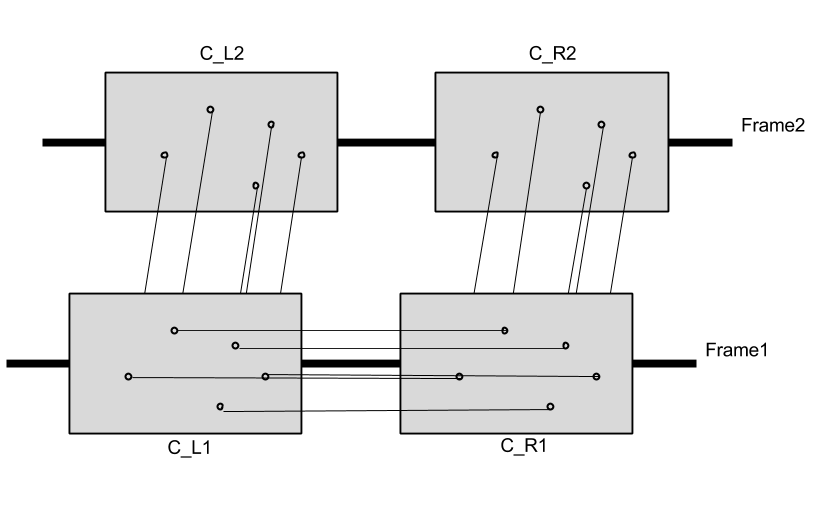
\includegraphics[width=0.7\textwidth]{images/image_setup.png}
		\caption{image setup}
	\end{figure}
	
	We start to detect features in $C_{L1}$ with the Shi-Tomasi Corner detector that is implemented in OpenCV. The Shi-Tomasi approach is a faster and more stable modification of Harris Corner detector \cite{Shi-Tomasi_Wiki}. 

	Features are characterized by their gradiation and the direction of the gradiation. With analyzing the eigenvalues of Window pattern around a pixel is it possible to decide if the point is a corner, an edge or neither of them. 
	
	\begin{figure}[H]
		\centering
		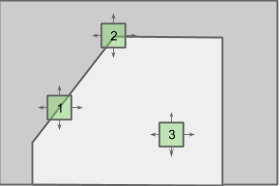
\includegraphics[width=0.65\textwidth]{images/tomasi.png}
		\caption{Shi-Tomasi approach}
	\end{figure}
	
	In figure 6 are shown different window pattern with different gradient. The first pattern is an edge because there is no change of gradient along the edge direction. Second pattern is a corner because there are changes in both directions. Last pattern has no change in any direction and is for this reason just classified as a flat surface (no feature) [\cite{Shi-Tomasi, FeatureDetection}. The Shi-Tomasi Corner detector is a really common approach, but an alternate could be the FAST feature detector or SURF (Speeded-Up Robust Features). 

	After finding the features in $C_{L1}$ the algorithm tries to find the corresponding points in $C_{R1}$ and $C_{L2}$. Subsequently the points found in $C_{R1}$ are matched with the ones of $C_{R2}$
	To refind points in different images we use the Lucas-Kanade algorithm that is also part of the OpenCV library.

	Beside SURF the Lucas-Kanade Algorithm is one of the most common methods to find features in an image. One requirement for this method is, that the intensity of a point in a specified window will not change from frame to frame. That is the main reason why the algorithm works best on systems with a high frame rate, so that the movement between the single frames is very low \cite{Lucas_Kanade}.

	In this project we used the pyramidical approach of this algorithm. Therefore the reference image is downscaled to a certain number of pyramidal layers (see figure 7) with different resolutions. Afterwards the Lucas-Kanade Algorithm is called on each layer in ascending order (only in the range found previously). Using this method the algorithm is way faster, more robust and provides a better accuracy \cite{Lucas_Kanade_TU_dresden}.

	\begin{figure}[H]
		\centering
		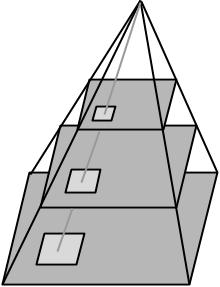
\includegraphics[width=0.3\textwidth]{images/pyramidical.png}
		\caption{pyramedical approach of Lucas-Kanade}
	\end{figure}
	
	In order to prevent wrong associations between points, outliers have to be deleted. Therefore OpenCV provides the findFundamentalMat() method using RANSAC \cite{findFundamentalMat}. Although the method is doing what it is supposed to do, it finds too many good points (inliers) and declares them as outliers, and vice versa. Because it is quiet difficult to retrace the wrong definition of points we have to define inliers manually. One good approach therefore is the constraint of having a rectified stereo camera system. The flow vectors between $C_{L1}$ and $C_{R1}$ as well as $C_{L2}$ to $C_{R2}$ have to be horizontal on the images (epipolar geometry). If that is not the case we delete this point in all four frames. The following figure shows the inliers, represented as green arrows as well as the outliers represented as red arrows.
	
	\begin{figure}[H]
		\centering
		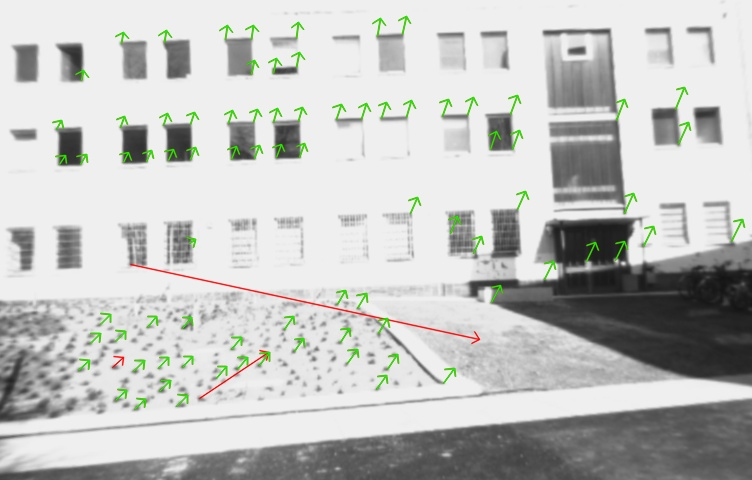
\includegraphics[width=0.6\textwidth]{images/inlier_outlier3.jpg}
		\caption{inliers (green) and outliers (red)}
	\end{figure}
	

	\section{Motion Estimation}
	
	Estimating motion between images is a hard task with many different approaches. Most of them use the projection matrix computed out of the essential matrix. The matrices we need are computed separately (left and right) between the current and the previous frame using detected features and correspondence points. First we need to compute the fundamental matrices for both sides using the findFundamentalMat method that is already implemented in OpenCV. Next we have to calculate the essential matrices using the camera matrices we get from the rectification using following formula \cite{HartleyZisserman}.
	\begin{align}
	  E = K’ \cdot F \cdot K
	\end{align}
	To obtain the perspective matrix we have to decompose the essential mat using SVD \cite{SVD_Essential}. Unfortunately the essential matrix can be decomposed to 4 different projection matrices and we have to find the right on. Therefore the points are triangulated using all four possible projection matrices with the goal to find the one where all points are in front of both cameras \cite{ComputerVision}.
	
	\begin{figure}[H]
		\centering
		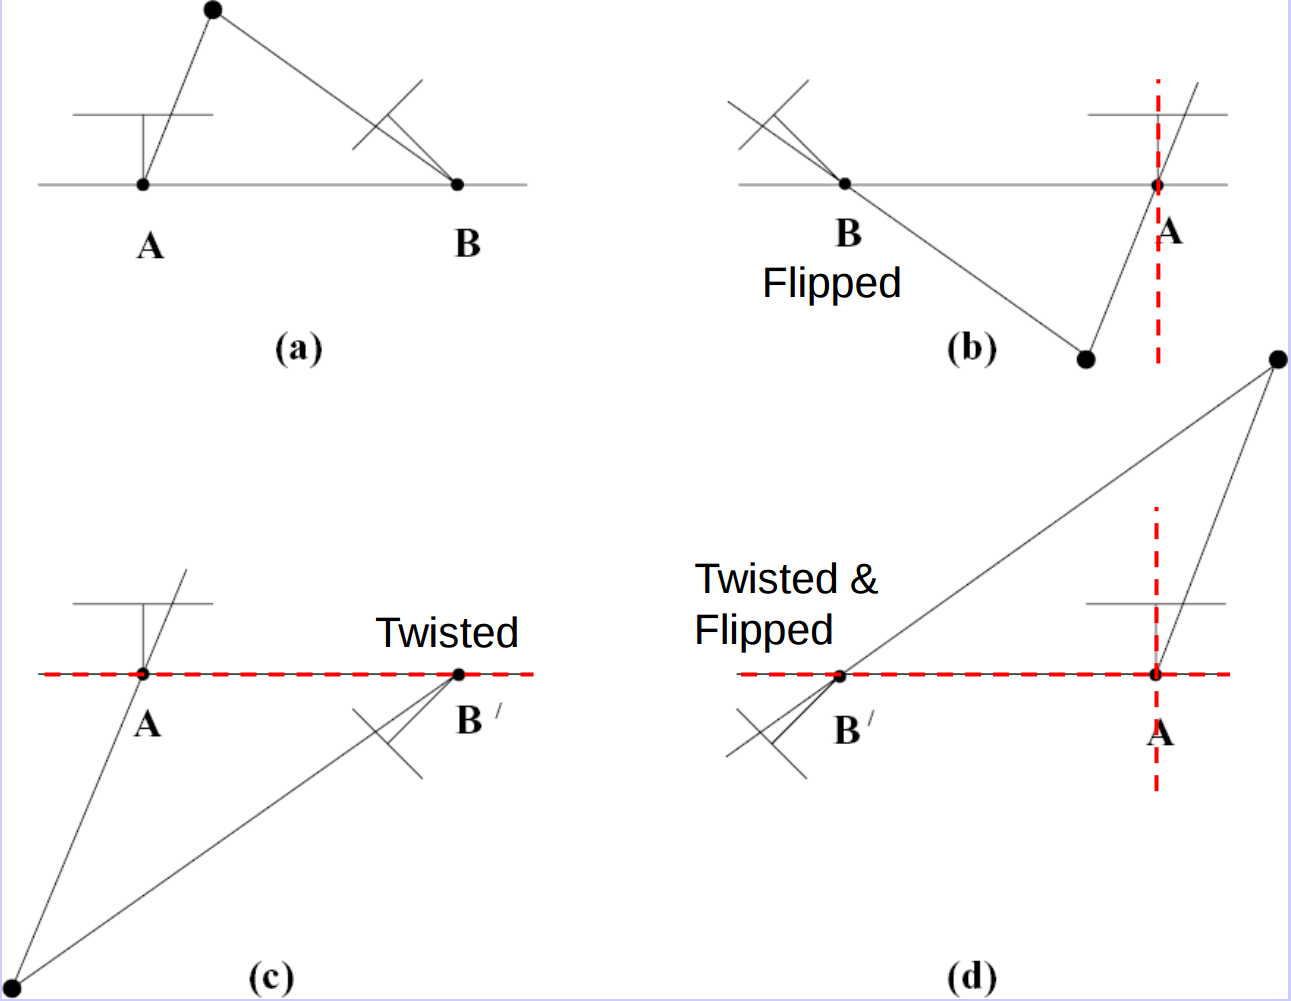
\includegraphics[width=0.6\textwidth]{images/possible_P_Mats.png}
		\caption{Decomposing of essential matrix \cite{ComputerVision}}
	\end{figure}

	One problem left is that the found projection matrix is up to scale, which basically means that we just get the normalized direction vector ($||T|| = 1$) and the rotation of each camera. In order to get the correct scale factors we have to triangulate a reference point cloud from the left to the right camera called $X$. This point cloud is in the right scale because it is computed using $P_{LR}$ which already contains metric values. Next we triangulate points from the previous left image to the current left image resulting $X_L$, the same procedure is used to calculate $X_R$. To estimate the scale factor for $L$ and $R$ we just compare the point clouds with the reference $X$ as the following formulas show \cite{scaleFactors}.
	\begin{align}
	  \mu = \frac{1}{n} * \sum_{i=1}^{n} \frac{\|X\|}{\|X_L\|} \qquad
	  \lambda = \frac{1}{n} * \sum_{i=1}^{n} \frac{\|X\|}{\|X_R\|}
	\end{align}

	Improving the estimation can be done by skipping frames where the motion estimation seems to fail and try to estimate the motion directly to the next valid frameset. To decide if the frameset is valid or not we can check against certain constraints. One of them is checking whether the determinant of $E$ is zero, the determinant of a valid rotation matrix should be either positive or negative one \cite{ValidEssential}. To determine a good fundamental matrix we need a minimum number of detected inliers. Also we defined a maximum motion per frame as a maximum of one meter, because moving more than one meter with a frame rate of either 30fps (binned) or 60fps is not realistic and can be declared as wrong. If one of this constraints cannot be fulfilled we skip the frameset and check the next one always remembering the last valid frameset. The method is robust as long we do not skip more than 4 frames because finding corresponding points after 4 frames is hard and if there is a circular motion nearly impossible. 

	\begin{figure}[H]
		\centering
		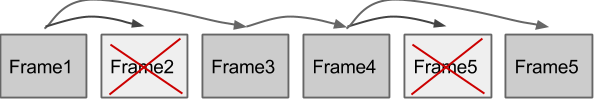
\includegraphics[width=0.7\textwidth]{images/skipFrames.png}
		\caption{approach of skipping frames}
	\end{figure}
	
	As described above there exist a lot of methods in the field of visual odometry. Beside the presented one we implemented two other approaches.
	The Perspective-n-point method is another way to estimate motion using a stereo-vision system. Therefore we have to find 3D-point to 2D-image-point correspondences. These are easy to gather using triangulation. Fortunately this method is included as RANSAC in OpenCV. The main idea is to use the dependency between 2D and corresponding 3D points. 2D points are here described as the multiplication of the projection matrix and the 3D points as explained in the following formula \cite{PnP}.
	\begin{align}
	  x_i = P * X_i \qquad x_i := \text{2D points} \\
	  \qquad X_i := \text{3D points} \nonumber
	\end{align}
	
	Second approach is to compare the orientation of the point cloud triangulated in frame i-1 to the point cloud triangulated in frame i (see figure [11]).
	The whole method is explained in the paper "Combining Stereo Vision and Inertial Navigation System" \cite{cloudOrientation} and is reimplemented by us.

	\begin{figure}[H]
		\centering
		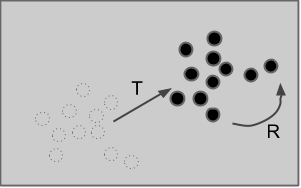
\includegraphics[width=0.5\textwidth]{images/pointcloud_orientation.png}
		\caption{approach of pointclout orientation}
	\end{figure}
	
	\section{Results}
	Using the first approach we gathered some useful results. We used the stereosystem connected to a notebook and walked around the Digital-Bauhaus-Lab in Weimar. Visually the estimated path matches to the one we walked. But as we take a deeper look on the results we can see that the start and end position is not matching though the test began and end in the exact same location. To express the added error in numbers we can take a look at the coordinates estimated. We started at [0, 0, 0] and stopped at [-0,23m, -5.46m, -1.9m], which means we drifted by $\pm$ 6m in every direction. At this point we were not able to gather any useful results using the other two approaches.
	
	\begin{figure}[H]
		\centering
		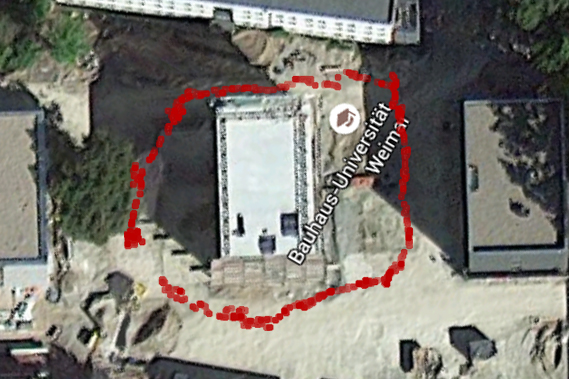
\includegraphics[width=0.5\textwidth]{images/result.jpg}
		\caption{path around the DBL in Weimar}
	\end{figure}

	\section{Issues}

	There are many different factors for good results when trying to estimate the motion out of stereo camera images. Obviously the corresponding points and their accuracy are the most important factor. The quality as well as the distribution of points are two very important components, but also the number of correct points. For a good triangulation it is essential that the found features are not too far away e.g at the horizon. The reason for that is the small distance between the points, so it is really hard to differ which feature belongs to another within different frames and camera images. Whereby the same problem occurs with too small translation. Another issue which can lead to problems is the size of the baseline between the cameras. If it is too small the triangulation might fail because of very low angles, if it is too big the number corresponding points can be to less.
	
	
	\section{Future work}
	In order to make the algorithm more robust it is important that the error from frame to frame does not grow more. Bundle adjustment could be a useful approach to solve this problem. A comparison between these three methods would be useful to evaluate the best method for a specific setup. Another idea would be to combine the methods to get a system which is able to cope with very different situations. The current code is basically written to be used in a comfortable way, therefore an implementation with focus on performance and stability would be important. Live test should be also done in order to evaluate the current performance and robustness.

	\newpage
	\bibliography{reference}

\end{document}